%!TEX encoding = UTF-8 Unicode
\documentclass[t,aspectratio=169,table]{beamer}
% Option t              Place text of slides at the (vertical) top of the slides.
% Option handout        Ein PDF ohne Pausen und Overlayeffekte erzeugen.
% Option aspectratio=43 169 => 16:9, 1610 => 16:10, 43 => 4:3
\usepackage[utf8]{inputenc}
\usepackage[ngerman]{babel}
\usepackage{graphicx,xcolor}
\usepackage[T1]{fontenc} % 8-Bit-Zeichen; ermöglicht korrektes Kopieren von Umlauten aus dem pdf

% SVS-Theme benutzen
\usetheme{svs2021}

\usepackage{booktabs}

\setlength{\arrayrulewidth}{0.1mm}
\setlength{\tabcolsep}{4pt}
% \renewcommand{\arraystretch}{1.5}
\renewcommand{\arraystretch}{1}

\usepackage[
    style=alphabetic,
    backend=biber,
    %backref=true
    ]{biblatex}             % Biblatex mit alphabetischem Style und biber.

\addbibresource{thesis.bib}

\DeclareFieldFormat*{title}{
    \mkbibemph{#1}}         % Make titles italics


% ===================================Dokument===================================


% \title{On using privacy preseving machine learning for\\decentralized web bot detection}
\title{On Machine Learning Based Bot Detection Using Mouse Dynamics and Request Metadata in a Practical Context}
\author{Matz-Jona Radloff}
\date{22.09.2022} % Falls ein bestimmtes Datum eingesetzt werden soll, einfach
                    %  diese Zeile aktivieren.
%\usepackage{pgfpages}
\begin{document}


%\pgfpagesuselayout{4 on 1}[a4paper,border shrink=5mm,landscape]

\section{Bachelor Thesis}
\begin{frame}
\maketitle
\end{frame}

\section{Outline}
\begin{frame}[allowframebreaks]
\frametitle{Outline}

\tableofcontents[sections={3-5}]
\framebreak
\tableofcontents[sections={6-20}]
%\framebreak
%\tableofcontents[sections={6-20}]

\end{frame}

\section{Introduction}

\subsection{Motivation}
\begin{frame}
\frametitle{Motivation}

\begin{itemize}
    \item (web) bot detection
    \item evaluate performance of mouse dynamics data vs. request metadata
    \item realistic conditions
    \item goal of being practical
\end{itemize}

\end{frame}

\subsection{Bot Detection Background}
\begin{frame}
\frametitle{Bot Detection Background}

\begin{itemize}
    \item differentiate human from computer automated actors
    \item here, web bots are defined as software that automatically performs HTTP(S) request to gather information or reach a goal
    \item deny bots with malicious intentions, e.g.
    \begin{itemize}
        \item Denial of Service (DoS)
        \item Data Scrapers
        \item Content Spam
        \item Scalping
    \end{itemize}
    \item \textbf{27.7\%} of all 2021 internet traffic generated by malicious bots \cite{BAD_BOT_REPORT2022}
    \item good bot traffic (14.6\%) desired to be allowed (e.g. search engine index bots)
    \item false positive intolerant
\end{itemize}

\end{frame}

\section{Related Work}

\subsection{Previous Works}
\begin{frame}
\frametitle{Previous Works}

\begin{itemize}
    \item Iliou et al. \cite{10.1145/3339252.3339267} compare different machine learning algorithms on request metadata
    \begin{itemize}
        \item request data from MK-Labs's public web server\footnote{Multimedia Knowledge and Social Media Analytics Laboratory, \url{https://mklab.iti.gr/}}
        \item ranking of derived features, e.g. percentage of image requests, number of bytes per session
        \item best machine learning methods are Random Forest and Multilayer Perceptron
        \item simple vs advanced bots, AUC of 1.00 and 0.64 (FPR 0.01 and 0.4)
    \end{itemize}
    \item Acien et al. \cite{Acien2020BeCAPTCHAMouseSM} use biometric features in a ML system for bot detection
    \begin{itemize}
        \item GAN-base mouse trajectory synthesis for training and evaluation
        \item Random Forest best ML algorithm in comparison
        \item 98.7\% accuracy
    \end{itemize}
    %\item Several works showed the potential viability of user authentication via mouse dynamics
\end{itemize}

\end{frame}

\subsection{Requirements and Contributions}
\begin{frame}
\frametitle{Requirements and Contributions}

\begin{itemize}
    \item directly comparable dataset and ML systems using request metadata and mouse dynamics data
    \item real world conditions
    \begin{itemize}
        \item many previous works' data collection and/or evaluation in lab setting
    \end{itemize}
    \item good performance (low FPR weighed highest) and execution speed
    \item above requirements have been shown to be viable separately but not together in a realistic setting
    \item proof of concept for practical application
\end{itemize}

\end{frame}

\section{Method}

\subsection{Request Metadata and Mouse Dynamics for Bot Detection}
\begin{frame}
\frametitle{Method}
\framesubtitle{Request Metadata and Mouse Dynamics for Bot Detection}

\begin{columns}
\column{0.4\textwidth}
\begin{itemize}
    \item comparison of mouse and touch data to request metadata
    \item mouse data contains a lot of information and are harder to fake
    \item big part of request metadata redundant, e.g. user agent
\end{itemize}

\column{0.6\textwidth}
\begin{figure}
    \includegraphics[width=\textwidth]{figures/user_mouse_heatmap.png}
    \caption{Mouse movements captured from a human user}
    %\label{fig:user_mouse_heatmap}
\end{figure}

\end{columns}

\end{frame}

\begin{frame}
\frametitle{Request Metadata and Mouse Dynamics for Bot Detection}

\begin{itemize}
    \item ML-based system: good performance and privacy friendliness
    \item only binary classification (only bot or human)
    \item smaller set of input features $\rightarrow$ increase execution speed and reduce complexity
    \item dataset collected and bot data generated using real websites
    \item comparison to existing dataset from Antal et. al's publication \cite{9111596}
\end{itemize}

\end{frame}

\subsection{Machine Learning Model}
\begin{frame}
\frametitle{Machine Learning Model}

Previous works showed that the Random Forest algorithm performs best for both data types
\begin{itemize}
    \item supervised ML algorithm
    \item ensemble of decision trees (reduces overfitting compared to single tree)
    %\item decision tree nodes split data according to a binary decision criterion
    %\item bagging of input data (per tree and node)
    %\item tree's results are averaged for final prediction
    %\item variable parameters (\# trees, \# features per tree, max tree depth, etc)
\end{itemize}

\begin{figure}[H]
    \includegraphics[width=0.7\textwidth]{figures/random_forest.png}
    \caption{Mouse movements captured from a human user}
    \label{fig:user_mouse_heatmap}
\end{figure}

\end{frame}

\subsection{Request Data Feature Selection}
\begin{frame}
\frametitle{Request Data Feature Selection}

\begin{itemize}
    \item Iliou et al. \cite{10.1145/3339252.3339267} ranked the best performing metrics
    \item the following, most applicable, subset is used
    \begin{itemize}
        \item \% of HTTP requests that returned 4xx, CSS or JS files
        \item \% of URLs that contain previous URL parts
        \item session length in seconds
        \item SD of requested pages' depth (i.e. number of '/' in URL)
        \item mean and SD of times between successive requests
    \end{itemize}
\end{itemize}

\end{frame}

\subsection{Mouse Data Feature Selection}
\begin{frame}
\frametitle{Mouse Data Feature Selection}

\begin{itemize}
    \item grouped into paths (click at the end, max 50 datapoints or 2 seconds long)
    % \item resampled such that all values or uniformly spaced in time (every 20ms)
    \item derived features are engineered similar to Gamboa et.al.\cite{GAMBOA2004} and \cite{https://doi.org/10.1049/iet-bmt.2018.5126}
    \begin{itemize}
        \item mean, SD, min, max, max-min computed for the following vectors
        \begin{itemize}
            \item path length
            \item angle with the $x$-axis
            \item horizontal, vertical, tangential and angular velocities
            \item tangential acceleration and jerk
        \end{itemize}
        \item total time, distance, straigtness, jitter \\
    \end{itemize}
    $\rightarrow$ 49 values
\end{itemize}

\end{frame}

\subsection{Websites for Data Collection}
\begin{frame}
\frametitle{Websites for Data Collection}

\begin{itemize}
    \item two blog-style websites with login and register functionality
    \item randomly generated content
    \item hybrid between classical and SPA approach
    \item both request and mouse data recorded in parallel (by JavaScript and Python backend)
    \item recorded data + UUID + human/bot label stored in database
\end{itemize}

\end{frame}

\begin{frame}
\frametitle{Websites for Data Collection}
\begin{centering}
\begin{figure}
    \includegraphics[width=0.8\textwidth]{screenshots/fmexp1_169.png}
    \caption{The user experiment's first website}
    \label{screenshot:fmexp1}
\end{figure}
\end{centering}
\end{frame}


\subsection{Bot Data Generation}
\begin{frame}
\frametitle{Bot Data Generation}

\begin{itemize}
    \item selenium-python and puppeteer (JavaScript) libraries used for automation
    \item different screen sizes, random pauses between actions, random order of actions
    \item request, mouse and advanced mouse bots implement the following actions
    \begin{itemize}
        \item Accepting the initial prompt dialog to start the experiment
        \item Visiting the top-level pages
        \item Visiting randomly selected (sub-)pages
        \item Registering an account
    \end{itemize}
\end{itemize}

\end{frame}

\begin{frame}
\frametitle{Bot Data Generation}

\begin{columns}
\column{0.4\textwidth}
\begin{itemize}
    \item mouse bots use actual mouse movements and clicks
    \item advanced mouse bot uses bezier curve interpolation of mouse trajectories
\end{itemize}

\column{0.6\textwidth}

\begin{figure}[h]
    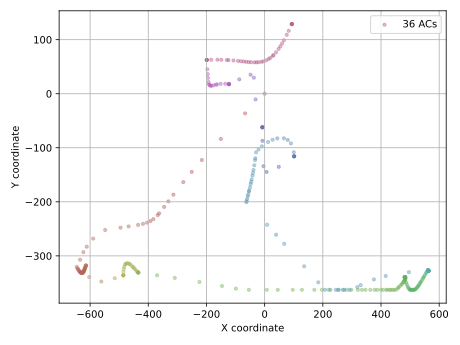
\includegraphics[width=\textwidth]{figures/bot_mouse_heatmap.png}
    \caption{Advanced Bot Mouse Movements Example}
    \label{fig:bot_mouse_heatmap}
\end{figure}
\end{columns}
\end{frame}

\section{Evaluation}

\subsection{Dataset}
\begin{frame}
\frametitle{Evaluation}
\framesubtitle{Dataset}

\begin{itemize}
    \item 322 and 163 users participated in the experiment
    \item maximum of 10 datapoints per session as a compromise between availability and performance
\end{itemize}

\begin{figure}[h]
    \includegraphics[width=0.9\textwidth]{figures/user_dp_hist.png}
    \caption{Distribution of users in terms of data point count}
    \label{fig:user_dp_hist}
\end{figure}

\end{frame}

\subsection{Model Hyperparameters}
\begin{frame}
\frametitle{Model Hyperparameters}

An empirical search determined the best combination of the following parameters:

\begin{itemize}
    \item Maximum number of features
    \item Number of estimators
    \item Maximum tree depth
\end{itemize}
The best parameters for request data were:
\begin{table}
    \begin{center}
        \begin{tabular}{lrlrrrrr}
            Max Features & \# Trees & Max Depth & Acc. & Prec. & Recall & AUC & Tr. Time (s) \\
            \midrule
            None & 100 & None & 0.910 & 0.887 & 0.940 & 0.973 & 0.486 \\
        \end{tabular}
    \end{center}
    \caption{Model accuracy for different parameters (request data)}
    \label{table:request_params}
\end{table}
The best parameters for mouse data were:
\begin{table}
    \begin{center}
        \begin{tabular}{lrlrrrrr}
            Max Features & \# Trees & Max Depth & Acc. & Prec. & Recall & AUC & Tr. Time (s) \\
            \midrule
            \rowcolor{green!30}
            sqrt & 200 & None & 0.966 & 0.962 & 0.970 & 0.994 & 5.899 \\
        \end{tabular}
    \end{center}
    \caption{Model accuracy for different parameters (mouse data)}
    \label{table:mouse_params}
\end{table}

\end{frame}


\subsection{Mouse Dynamics Data Compared to Request Metadata}
\begin{frame}
\frametitle{Mouse Dynamics Data Compared to Request Metadata}
\framesubtitle{Results}

\begin{itemize}
    \item Mouse data performs better than request metadata
    \item Every 26th vs. every 8th human would be classified as a bot
    \item Both data types combined:
    \begin{itemize}
        \item mouse data results averaged per user for direct comparison
        \item \textbf{96\%} accuracy, 0 FPR
    \end{itemize}
\end{itemize}

\begin{table}[H]
    \begin{center}
        \begin{tabular*}{\textwidth}{l @{\extracolsep{\fill}} rrrr}
            Data Type & Accuracy & AUC & FPR & FNR \\
            \midrule
            Mouse data & 96.6\% & 0.973 & 0.04 & 0.03 \\
            Request metadata & 91\% & 0.994 & 0.12 & 0.06 \\
            Mouse+Request (0.1 split) & 96\% & 0.976 & 0 & 0.05 \\
            Mouse+Request (0.2 split) & 95\% & 0.970 & 0 & 0.06 \\
        \end{tabular*}
    \end{center}
    \caption{Simple and Advanced Mouse Data Performance}
    \label{table:simple_vs_advanced_mouse}
\end{table}

\end{frame}

\subsection{Simple and Advanced Mouse Bot Data Generation}
\begin{frame}
\frametitle{Simple and Advanced Mouse Bot Data Generation}
\framesubtitle{Results}

\begin{itemize}
    \item All available human data and simple vs advanced bot data for training
    \item High accuracy, low FPR
    \item simple bots can be very easily identified
\end{itemize}

\begin{table}[H]
    \begin{center}
        \begin{tabular*}{\textwidth}{l @{\extracolsep{\fill}} rrrrr}
            Scenario & Accuracy & Precision & Recall & AUC & Training Time (s) \\
            \midrule
            Basic mouse bot & 0.995 & 0.997 & 0.994 & 1.000 & 0.857 \\
            Advanced mouse bot & 0.966 & 0.962 & 0.970 & 0.994 & 1.293 \\
        \end{tabular*}
    \end{center}
    \caption{Simple and Advanced Mouse Data Performance}
    \label{table:simple_vs_advanced_mouse}
\end{table}


\end{frame}

\subsection{Does the Trained ML Model Generalize?}
\begin{frame}
\frametitle{Does the Trained ML Model Generalize?}
\framesubtitle{Results}

\begin{itemize}
    \item Different datasets for training and testing
    \item Basic <> Advanced, Website 1 <> Website 2
\end{itemize}

\begin{table}[H]
    \begin{center}
        \begin{tabular*}{\textwidth}{l @{\extracolsep{\fill}} rrrrrr}
            Scenario & Accuracy & Precision & Recall & AUC & Training Time \\
            \midrule
            Basic tr. data, adv. test data & 0.529 & 0.952 & 0.061 & 0.765 & 0.888 \\
            Adv. tr. data, basic test data & 0.769 & 0.938 & 0.577 & 0.928 & 1.306 \\
            W1 training data, W2 test data & 0.966 & 0.955 & 0.964 & 0.993 & 1.075 \\
            W2 training data, W1 test data & 0.914 & 0.715 & 0.961 & 0.983 & 0.524 \\
        \end{tabular*}
    \end{center}
    \caption{Model performance with separate training and test data}
    \label{table:simple_vs_advanced_mouse_separate_train_test}
\end{table}

\begin{itemize}
    \item Training with only basic or advanced bot data does not generalize well
    \item Training with Website 1 data performs better because it has more datapoints
\end{itemize}

\end{frame}

\subsection{Comparison to External Dataset}
\begin{frame}
\frametitle{Comparison to External Dataset}
\framesubtitle{Results}

\begin{itemize}
    \item Comparison to Antal et. al's dataset \cite{9111596}
    \begin{itemize}
        \item Raw mouse and touchpad data from 21 users
        \item $151M$ datapoints, $1.54M$ input vectors
    \end{itemize}
    \item Training with data from both websites and advanced bots
    \item \textbf{82.25\%} accuracy, \textbf{22.13\%} FPR (one user)
    \item \textbf{83.03\%} accuracy, \textbf{17.16\%} FPR (all users)
    \item Very unbalanced because dataset only contains human data
    \item \textbf{99.71\%} accuracy, \textbf{0.55\%} FPR when training on ext. dataset
\end{itemize}

\end{frame}

\subsection{Execution Speed and Performance?}
\begin{frame}
\frametitle{Execution Speed and Performance?}

\begin{columns}
\column{0.3\textwidth}
\begin{itemize}
    \item \textbf{$27ms$} with only 100 previous data points (\textbf{93.67\%} acc.)
    \item $23.78ms$ experiment's websites average response time
    \item run asynchronously and/or optimize code
\end{itemize}

\column{0.7\textwidth}
\begin{centering}
\begin{figure}
    \includegraphics[width=\textwidth]{figures/speed_per_dp_count.png}
    \caption{Execution speed and score versus number of previous data points}
    \label{fig:speed_per_dp_count}
\end{figure}
\end{centering}

\end{columns}

\end{frame}

\section{Conclusion}
\begin{frame}
\frametitle{Conclusion}
\begin{itemize}
    \item ML-based bot detection system using pointer data is practically viable
    \item performance good enough for some use cases
    \item execution speed acceptable if optimized or run asynchronously
    \item better performance can be traded for speed
    \item good addition to existing solutions
    \item only possible if pointer data available (request data as fallback)
\end{itemize}
\end{frame}

\section{Bibliography}
\begin{frame}[allowframebreaks]
\frametitle{Bibliography}

\begin{raggedright}
  \printbibliography
\end{raggedright}

\end{frame}

%\begin{frame}[allowframebreaks]

%\end{frame}

\end{document}
